\section{Механические колебания}
%TODO разделы
%TODO задача краевой олимпиады 2007


%-----------------Пружинный маятник---------------------
%Ландау
\begin{ex}
\hspace{0pt} \\
\begin{minipage}{.65\textwidth}
Найдите частоту колебаний точки с массой $m$, способной двигаться по прямой и прикрепленной к пружине, другой конец которой закреплен в точке $A$ на расстоянии $l$ от прямой. Пружина, имея длину $l$, натянута с силой $F$.
\end{minipage}
\begin{minipage}{.35\textwidth}
\centering
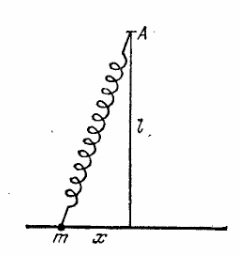
\includegraphics[width = 0.5 \textwidth]{1303OscillationsSpringAndLine.jpg}
\end{minipage}
\begin{ans}
$\omega = \sqrt{F/ml}$
\end{ans}
\end{ex}

%Ландау
\begin{ex}
\hspace{0pt} \\
\begin{minipage}{.65\textwidth}
Найдите частоту колебаний точки с массой $m$, способной двигаться по окружности радиуса $r$ и прикрепленной к пружине, другой конец которой закреплен в точке $A$, кратчайшее расстоянии то точки $A$ до окружности равно $l$. Пружина, имея длину $l$, натянута с силой $F$.
\end{minipage}
\begin{minipage}{.35\textwidth}
\centering
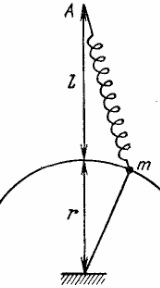
\includegraphics[width = 0.5 \textwidth]{1304OscillationsSpringAndCircle.jpg}
\end{minipage}
\begin{ans}
$\omega = \sqrt{\frac{F(r+l)}{rml}}$
\end{ans}
\end{ex}

\begin{ex}
\hspace{0pt} \\
\begin{minipage}{.65\textwidth} 
(2007) С какой частотой $\omega_0$ будет совершать малые вертикальные колебания в поле тяжести груз массы $m$, подвешенный на двух одинаковых пружинах жесткости $k$, образующих в равновесии углы $\beta$ с вертикалью?
\end{minipage}
\begin{minipage}{.35\textwidth}
\centering
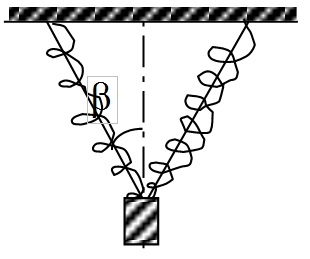
\includegraphics[width = 0.7 \textwidth]{132007OscillationsTwoSpringsAndWeight.jpg}
\end{minipage}
\begin{ans}
$\omega = \cos \beta \sqrt{2k/m}$
\end{ans}
\end{ex}

%Иродов-3.51
\begin{ex}
\hspace{0pt} \\
\begin{minipage}{.65\textwidth} 
Найти круговую частоту малых колебаний тонкого стержня массы $m$ и длины $l$ вокруг горизонтальной оси, проходящей через точку $O$. 
Жесткость пружины $k$. В положении равновесия стержень вертикален.
\end{minipage}
\begin{minipage}{.35\textwidth}
\centering
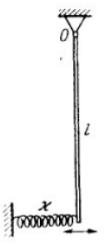
\includegraphics[width = 0.2 \textwidth]{SpringRodOsc.png}
\end{minipage}
\begin{ans}
$\omega = \sqrt{3g/2l+3k/m}$
\end{ans}
\end{ex}

\begin{ex}
\hspace{0pt} \\
\begin{minipage}{.65\textwidth}
(2016) Студент университета Пружинкин, увлекающийся физическим экспериментом (и не очень любящий теорию) смонтировал в физической лаборатории маятник. Маятник представлял собой очень легкий шарнирно закрепленный стержень длины $l = 50$ см (шарнир в нижней точке стержня), на котором были закреплены два одинаковых шарика c массами по $m = 0,9$ кг: один шарик -- в середине стержня, a другой нa верхнем его конце. Между стержнем и вертикальной неподвижной стенкой на высоте $h=3l/4$ от шарнира студент закрепил горизонтальные пружинки различной жесткости. В положении равновесия деформация пружинок была равна нулю. Для того, чтобы построить экспериментальный график зависимости периода малых колебаний от жесткости, студент изготовил для опытов пять пружинок с известными жесткостями $k = 10, 20, 30, 40, 50$ Н/м. Выведите выражение для периода колебаний маятника и предскажите результаты опытов Пружинкина.
\end{minipage}
\begin{minipage}{.35\textwidth}
\centering
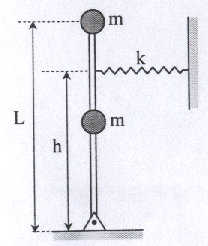
\includegraphics[width = 0.9 \textwidth]{InvertedPenduumWithSpring.png}
\end{minipage}
\begin{ans}
$T=2\pi \sqrt{\frac{20ml}{9kl-24mg}}$, при $k>24mg/9l$
\end{ans}
\end{ex}

\begin{ex}
(2015) На гладкой горизонтальной поверхности находится грузик, прикрепленный двумя одинаковыми пружинами к стенкам (рис. 2, вид сверху). 
В положении равновесии грузика пружины имеют одинаковое растяжение~$\Delta l$. 1) В первом случае груз совершает малые колебания вдоль оси~$x$. 
Как зависит период этих колебаний от величины~$\Delta l$?   2) Во втором случае траектория грузика, совершающего малые колебания, изображена на рис. 3 (в увеличенном виде).
Определите $\Delta l$, если длина пружин в нерастянутом состоянии $l$~=~15 см. Во всех случаях выполняется закон Гука.
\begin{center}
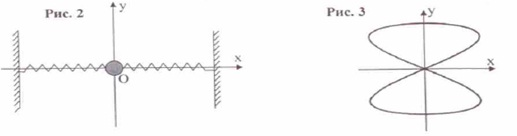
\includegraphics[width = 0.7 \textwidth]{132015OscillationsLissajousCurve.jpg}
\end{center}
\begin{ans}
$\omega_x = \sqrt{2k/m}$, $\omega_y=\sqrt{\frac{2k\Delta l}{m(l+\Delta l)}}$, $\Delta l = l/3$
\end{ans}
\end{ex}

%Ижевск
\begin{ex}
\hspace{0pt} \\
\begin{minipage}{.65\textwidth}
Схема динамического поглотителя колебаний представлена на рисунке. На первую массу действует гармоническая сила $F(t)~=~F_0\,\sin\,\omega\,t$. 
При каких условиях амплитуда вынужденных колебаний первой массы будет равна нулю?
\end{minipage}
\begin{minipage}{.35\textwidth}
\centering
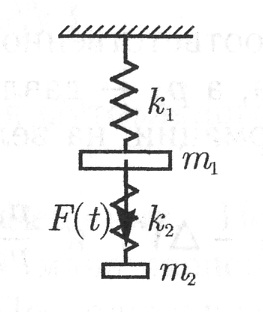
\includegraphics[width = 0.5 \textwidth]{1302OscillationsDynamicAbsorbentOfOscillations.jpg}
\end{minipage}
\begin{ans}
$\omega = \sqrt{k_2/m_2}$
\end{ans}
\end{ex}

%Черепанов
\begin{ex}
Груз массой $m$ прикреплен к пружине жесткостью $k$, а пружина к точке подвеса. 
Под действием внешней силы точка подвеса колеблется в вертикальном направлении по закону $x_p~=~A~\cos\,\omega t$. 
Какова амплитуда установившихся колебаний груза в вязкой среде, если сила сопротивления пропорциональна скорости $(F~=~-bv)$?
\begin{ans}
$x^2 = A^2\frac{\omega_0^4+4\beta^2\omega^2}{(\omega_0^2-\omega^2)^2+4\beta^2\omega^2}$, $\omega_0 = \sqrt{k/m}$, $\beta = b/2m$
\end{ans}
\end{ex}

%-------------Колебания газа в банке---------------
%Бутиков
\begin{ex} Расположенный горизонтально цилиндрический сосуд объема $V$, заполненный $\nu$ молями идеального газа, 
разделен поршнем массы $m$, который может двигаться без трения. В равновесии поршень находится посередине цилиндра. 
При малых смещениях из положения равновесия поршень совершает колебания. Найдите зависимость частоты этих колебаний от температуры, 
считая процесс изотермическим. Площадь поперечного сечения трубки равна~$S$.
\begin{ans}
$\omega^2=\frac{2\nu R S^2}{mV^2}T$
\end{ans}
\end{ex}

%Ижевск
\begin{ex}
\hspace{0pt} \\
\begin{minipage}{.65\textwidth} 
В длинной вертикальной цилиндрической трубке, закрытой с нижнего конца, может ходить без трения поршень, 
масса $M$ которого велика по сравнению с массой газа, заключенного внутри трубки. В положении равновесия расстояние между поршнем и дном трубки равно $L$. 
Определить период малых колебаний, которые возникнут при отклонении поршня от положения равновесия, в предположении, что они являются изотермическими, 
а газ идеальным. Площадь поперечного сечения трубки равна $S$, атмосферное давление равно $P_0$. Рассмотреть предельный случай, когда $P_0$~=~0.
\end{minipage}
\begin{minipage}{.35\textwidth}
\centering
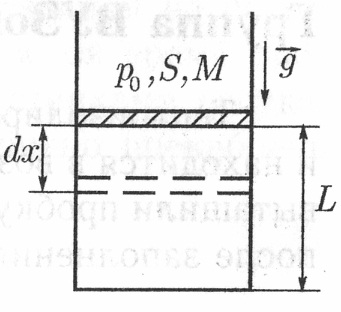
\includegraphics[width = 0.9 \textwidth]{1308OscillationsPistonInVerticalTube.jpg}
\end{minipage}
\begin{ans}
$T=2\pi\sqrt{\frac{ML}{p_0S + Mg}}$
\end{ans}
\end{ex}

%-----------Колебания жидкости-------------
%Иродов-3.20
\begin{ex}
\hspace{0pt} \\
\begin{minipage}{.65\textwidth} 
Идеальная жидкость объема $V$ налита в изогнутую трубку с площадью сечения канала $S$. Найти период малых колебаний жидкости.
\end{minipage}
\begin{minipage}{.35\textwidth}
\centering
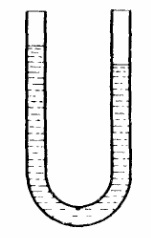
\includegraphics[width = 0.3 \textwidth]{1310OscillationsPerfectLiquid.jpg}
\end{minipage}
\begin{ans}
$T=\pi \sqrt{2V/Sg}$
\end{ans}
\end{ex}

%Иродов-3.21
\begin{ex}
Трубка высотой $H$ наполнена жидкостью и соединена с наклонной трубкой (угол наклона к вертикали $\alpha$). Каков будет период колебаний жидкости в такой системе?
\begin{ans}
$T=2\pi \sqrt{H/g(1+\cos \alpha)}$
\end{ans}
\end{ex}

\begin{ex}
\hspace{0pt} \\
\begin{minipage}{.65\textwidth} 
(2006) В тонкой трубке может скользить без трения веревка длиной $L$. В начальный момент времени веревка находится в левом колене. 
Определить период колебаний $T$ веревки. Жесткостью веревки на изгиб пренебречь. 
Каким будет период колебаний $T_1$, если расстояние между вертикальными коленами трубки увеличить с $L$ до $2L$?
\end{minipage}
\begin{minipage}{.35\textwidth}
\centering
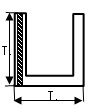
\includegraphics[width = 0.7 \textwidth]{132006OscillationsRopeInTube.jpg}
\end{minipage}
\begin{ans}
$T=2\pi\sqrt{L/g}$, $T=2(\pi+1)\sqrt{L/g}$
\end{ans}
\end{ex}

%-----------Затухающие колебания-------------

% Иродов-3.88
\begin{ex}
\hspace{0pt} \\
\begin{minipage}{.65\textwidth} 
Тонкий однородный диск массы $m$ и радиуса $R$, подвешенный в горизонтальном положении к упругой нити, совершает крутильные колебания в жидкости. 
Момент упругих сил со стороны нити $M~=~\alpha\,\varphi$.  Сила сопротивления на единицу поверхности $F~=~\eta\,v$. Найти частоту малых колебаний.
\end{minipage}
\begin{minipage}{.35\textwidth}
\centering
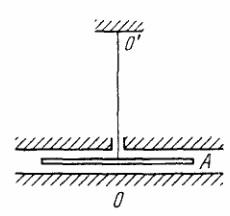
\includegraphics[width = 0.9 \textwidth]{1309OscillationsDisc.jpg}
\end{minipage}
\begin{ans}
$\omega = \sqrt{2\alpha/mR^2-(\pi \eta R^2/m)^2}$
\end{ans}
\end{ex}

%Черепанов
\begin{ex}
(2004) На горизонтальной плоскости с коэффициентом трения $\mu$ лежит брусок массы $m$, который пружиной жесткости $k$ соединен с вертикальной стенкой. Брусок сместили на расстояние $9\mu mg /2k$ и отпустили. Найти число колебаний бруска до остановки.
\begin{ans}
одно колебание
\end{ans}
\end{ex}

%------------Колебания в поле силы тяжести------------
\begin{ex}
\hspace{0pt} \\
\begin{minipage}{.65\textwidth} 
Найти период малых колебаний плоского маятника, точка подвеса которого с массой $M$ находится на гладкой горизонтальной прямой 
(масса маятника $m$ и его длина $L$).
\end{minipage}
\begin{minipage}{.35\textwidth}
\centering
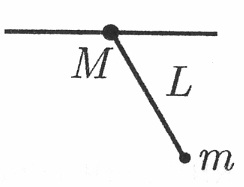
\includegraphics[width = 0.7 \textwidth]{1314OscillationsPlanePendulum.jpg}
\end{minipage}
\begin{ans}
$T=2\pi \sqrt{\frac{L}{g(1+m/M)}}$
\end{ans}
\end{ex}

%Ижевск
\begin{ex}
Дана проволочная вешалка, которая качается с малой амплитудой в плоскости рисунка относительно заданных положений равновесия. 
В положениях а и б длинная сторона вешалки расположена горизонтально. Две другие стороны равны между собой. 
Во всех трех случаях (а, б, в) возникают колебания с одинаковыми периодами. Где расположен центр масс вешалки?
\begin{center}
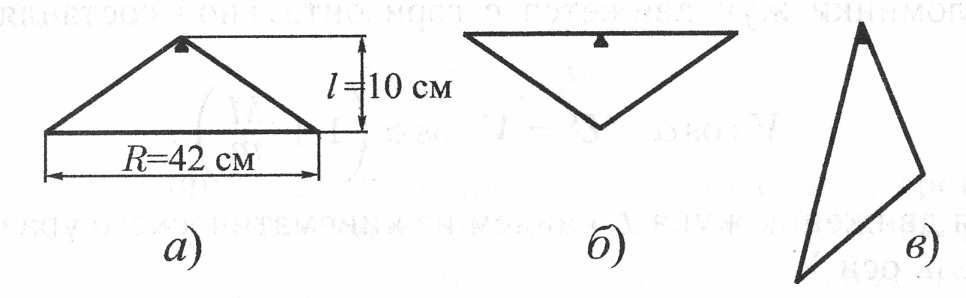
\includegraphics[width = 0.5 \textwidth]{1315OscillationsHanger.jpg}
\end{center}
\begin{ans}
На расстоянии 5 см от вершины треугольника
\end{ans}
\end{ex}

\begin{ex}
\hspace{0pt} \\
\begin{minipage}{.65\textwidth}
(2013) Точка подвеса математического маятника движется с постоянным ускорением $a$ (лежащим в плоскости колебаний маятника) в горизонтальном направлении. Найти закон движения маятника.
\end{minipage}
\begin{minipage}{.35\textwidth}
\centering
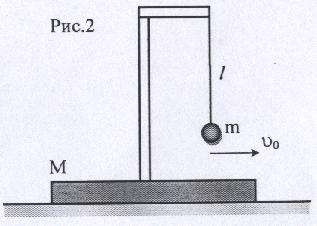
\includegraphics[width = 0.7 \textwidth]{PlatformWithOscillator.png}
\end{minipage}
\begin{ans}
$\alpha(t) = A \cos(\sqrt{\sqrt{a^2+g^2}/l}t) + \alpha_0$, $\alpha_0 = \arctan(a/g)$
\end{ans}
\end{ex}

\begin{ex}
(2017) Один конец однородного стержня длиной $L=1$ м закреплен на горизонтальной оси O (перпендикулярной плоскости чертежа), вокруг которой он может вращаться без трения. Другой конец стержня свободно лежит на опоре A, при этом стержень горизонтали. Свободный конец стержня приподнимают на высоту $h = 1$ см относительно исходного положения, поворачивая стержень
вокруг оси O, и отпускают бы начальной скорости. 1) Определите скорость
свободного конца стержня при ударе об опору А. 2) Определите частоту ударов
стержня об опору А, считая удары абсолютно упругими и мгновенными.
Ускорение свободного падения $g$ = 10 м/с\textsuperscript{2}. Трением пренебречь.
\begin{center}
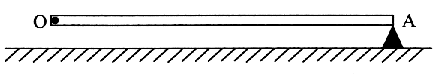
\includegraphics[width = 0.4 \textwidth]{HittingRod.png}
\end{center}
\begin{ans}
1) $v=\sqrt{3gh}$; 2) $\nu = 0.25\sqrt{3g/h }$
\end{ans}
\end{ex}

\begin{ex}
(2010) На абсолютно гибкой нити подвешен маятник. Расстояния до точки подвеса равны $S_1$ и $S_2$. 
Статический прогиб в точке подвеса маятника равен $y_0$, а длина маятника $l$, его масса $m$. 
Принять, что при $t$~=~0 точка подвеса имеет вертикальное смещение $A$, а ее скорость $v_0$ равна нулю; маятник отклонен на угол $\varphi_0$. 
Считая, что натяжение нити $T = T_0 = const$, вывести дифференциальное уравнение малых колебаний маятника.
\begin{center}
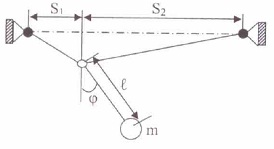
\includegraphics[width = 0.5 \textwidth]{132010OscillationsPendulumOnThread.jpg}
\end{center}
\begin{ans}
$ml \varphi^{\prime \prime} + (mg-m \omega^2 A \cos \omega t) \varphi = 0$, $\omega^2 = T_0(S_1+S_2)/m S_1 S_2$
\end{ans}
\end{ex}

\begin{ex}
(2014) В центре плоского конденсатора удерживают диполь в положении 1, указанном на рисунке. 
Диполь представляет собой два маленьких заряженных шарика с зарядами $q$ и $-q$ и массами $m$ каждый, 
соединенных невесомым непроводящим стержнем длины $L$. Разность потенциалов между пластинами конденсатора равна $U$, 
расстояние между пластинами равно $d$ (много меньше размеров пластин). Диполь поворачивают вокруг его центра и переводят в положение 2, 
которое является устойчивым положением равновесия диполя. 
1) Определите работу электрического поля при повороте диполя из положения 1 в положение 2. 
2) Определите период малых крутильных колебаний диполя вокруг положения 2. 
3) Какую минимальную скорость нужно сообщить диполю в положении 2 параллельно пластинам для того, чтобы диполь улетел из конденсатора? 
Силу тяжести не учитывать.
\begin{center}
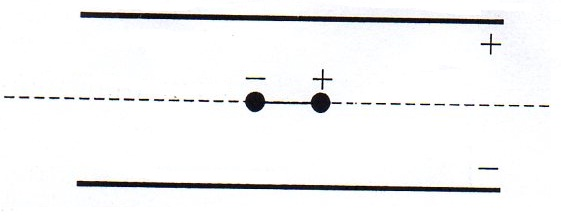
\includegraphics[width = 0.4 \textwidth]{132014OscillationsCondenserAndDoublet.jpg}
\end{center}
\begin{ans}
1) $A=qUL/d$; 2) $T=2\pi\sqrt{\frac{mLd}{2qU}}$; 3) $v_0 = \sqrt{\frac{qUL}{md }}$
\end{ans}
\end{ex}

\begin{ex}
Молекулу одноатомного газа массы $m$, совершающую колебания около некоторого положения равновесия с амплитудой $a$ и частотой $\omega$, 
в первом приближении можно считать линейным гармоническим осциллятором. 
Найти $f(x)$ -- функцию распределения вероятностей значений координаты $x$ такого осциллятора, среднее значение координаты $\langle x \rangle$, 
среднее значение $\langle U \rangle$ потенциальной энергии осциллятора.
\begin{ans}
\end{ans}
\end{ex}